\documentclass[hyperref={colorlinks=true}]{beamer}
\usepackage{amsmath,amsfonts,amsthm,amssymb}
\usepackage{mathrsfs}
% Not in French
%\usepackage[latin1]{inputenc}
%\usepackage[OT2,T1]{fontenc}
\usepackage[french]{babel}
\usepackage[utf8]{inputenc}
\usepackage[T1]{fontenc}
\usepackage{graphicx}
\usepackage{color}
\usepackage{xypic}\xyoption{tips}
\usepackage{pgfplots}
\usepackage{url}
\usepackage{calrsfs}
\usepackage{array}
\usepackage{tikz}
\usetikzlibrary{shadows,patterns,shapes}

%\usepackage{fourier}

\newtheorem{proposition}{{\bf Proposition}}[section]
    

%%%%%%%%%%%%%%%%%%%%%%%%%%%%%%%%%%%%%%%%%%%%%%%%%%%%%%%%%%%%%%%%%%%%%%%%%%%%%%
% Choose a theme:
%%%%%%%%%%%%%%%%%%%%%%%%%%%%%%%%%%%%%%%%%%%%%%%%%%%%%%%%%%%%%%%%%%%%%%%%%%%%%%
%\usetheme{Berlin}
%\usetheme{Copenhagen}
%\usetheme{Darmstadt}
%\usetheme{Marburg}
\usetheme{Singapore}
%\usetheme{Szeged}
%\usetheme{Warsaw}
%%%%%%%%%%%%%%%%%%%%%%%%%%%%%%%%%%%%%%%%%%%%%%%%%%%%%%%%%%%%%%%%%%%%%%%%%%%%%%
% Choose a color theme:
%%%%%%%%%%%%%%%%%%%%%%%%%%%%%%%%%%%%%%%%%%%%%%%%%%%%%%%%%%%%%%%%%%%%%%%%%%%%%%
\usecolortheme{crane}
%\usecolortheme{dove}
%\usecolortheme{dolphin}
%%%%%%%%%%%%%%%%%%%%%%%%%%%%%%%%%%%%%%%%%%%%%%%%%%%%%%%%%%%%%%%%%%%%%%%%%%%%%%
% Choose a font theme:
%%%%%%%%%%%%%%%%%%%%%%%%%%%%%%%%%%%%%%%%%%%%%%%%%%%%%%%%%%%%%%%%%%%%%%%%%%%%%%
\usefonttheme{structurebold}
%%%%%%%%%%%%%%%%%%%%%%%%%%%%%%%%%%%%%%%%%%%%%%%%%%%%%%%%%%%%%%%%%%%%%%%%%%%%%%
%%%%%%%%%%%%%%%%%%%%%%%%%%%%%%%%%%%%%%%%%%%%%%%%%%%%%%%%%%%%%%%%%%%%%%%%%%%%%%
\setbeamercovered{dynamic}

% Blackboard bold characters:
\renewcommand{\AA}{\mathbb{A}}
\newcommand{\FF}{\mathbb{F}}
\newcommand{\PP}{\mathbb{P}}
\newcommand{\NN}{\mathbb{N}}
\newcommand{\QQ}{\mathbb{Q}}
\newcommand{\RR}{\mathbb{R}}
\newcommand{\ZZ}{\mathbb{Z}}

% Caligraphic characters:
\newcommand{\cA}{\mathcal{A}}
\newcommand{\cB}{\mathcal{B}}
\newcommand{\cC}{\mathcal{C}}
\renewcommand{\cD}{\mathcal{D}}
\newcommand{\cE}{\mathcal{E}}
\newcommand{\cF}{\mathcal{F}}
\renewcommand{\cH}{\mathcal{H}}
\renewcommand{\cL}{\mathcal{L}}
\newcommand{\cM}{\mathcal{M}}
\newcommand{\cN}{\mathcal{N}}
\newcommand{\cO}{\mathcal{O}}
\newcommand{\cP}{\mathcal{P}}
\renewcommand{\cR}{\mathcal{R}}
\newcommand{\cS}{\mathcal{S}}
\newcommand{\cX}{\mathcal{X}}

\begin{document}

\title{Enveloppe's protocol Bitcoin based}
\author{Thomas Suau\newline
Universit\'e Libre de Bruxelles (ULB) }
\date{Brussels \newline May 24th, 2024}


%%%%%%%%%%%%%%%%%%%%%%%%%%%%%%%%%%%%%%%%%%%%%%%%%%%%%%%%%%%%%%%%%%%%%%%%
% TITLEPAGE
%%%%%%%%%%%%%%%%%%%%%%%%%%%%%%%%%%%%%%%%%%%%%%%%%%%%%%%%%%%%%%%%%%%%%%%%
\begin{frame}\titlepage\end{frame}
%%%%%%%%%%%%%%%%%%%%%%%%%%%%%%%%%%%%%%%%%%%%%%%%%%%%%%%%%%%%%%%%%%%%%%%%
%%%%%%%%%%%%%%%%%%%%%%%%%%%%%%%%%%%%%%%%%%%%%%%%%%%%%%%%%%%%%%%%%%%%%%%%

%%%%%%%%%%%%%%%%%%%%%%%%%%%%%%%%%%%%%%%%%%%%%%%%%%%%%%%%%%%%%%%%%%%%%%%%
% TABLE OF CONTENTS
%%%%%%%%%%%%%%%%%%%%%%%%%%%%%%%%%%%%%%%%%%%%%%%%%%%%%%%%%%%%%%%%%%%%%%%%
\begin{frame}\tableofcontents\end{frame}
%%%%%%%%%%%%%%%%%%%%%%%%%%%%%%%%%%%%%%%%%%%%%%%%%%%%%%%%%%%%%%%%%%%%%%%%
%%%%%%%%%%%%%%%%%%%%%%%%%%%%%%%%%%%%%%%%%%%%%%%%%%%%%%%%%%%%%%%%%%%%%%%%
%%%%%%%%%%%%%%%%%%%%%%%%%%%%%%%%%%%%%%%%%%%%%%%%%%%%%%%%%%%%%%%%%%%%%%%%
%%%%%%%%%%%%%%%%%%%%%%%%%%%%%%%%%%%%%%%%%%%%%%%%%%%%%%%%%%%%%%%%%%%%%%%%
% Short title:
\section{1. Why enveloppes?}
%%%%%%%%%%%%%%%%%%%%%%%%%%%%%%%%%%%%%%%%%%%%%%%%%%%%%%%%%%%%%%%%%%%%%%%%
%%%%%%%%%%%%%%%%%%%%%%%%%%%%%%%%%%%%%%%%%%%%%%%%%%%%%%%%%%%%%%%%%%%%%%%%

\begin{frame}
\frametitle{Pushing data on Bitcoin}

\begin{center}
{\Large The idea to push and retrieve data on Bitcoin is not young we call them {\bf metaprotocols}} :
\vspace{0.3cm}
\begin{itemize}

\item \href{https://yoniassia.com/coloredbitcoin/}{{\bf Colored Coins}}: A protocol to create and trade tokens on Bitcoin created in 2012; \\

\item \href{https://cryptochainuni.com/wp-content/uploads/Mastercoin-2nd-Bitcoin-Whitepaper.pdf}{{\bf Mastercoin}}: Same idea as Colored Coins but with one specific currency associated MSC which made the first {\it Initial Coin Offering} (ICO) in 2013;\\

\item \href{https://docs.counterparty.io/docs/basics/what-is-counterparty/}{{\bf Counterparty}}: A more general protocol created in January 2014 to allow complex contracts resolution on Bitcoin.\\

\end{itemize}

\end{center}

\end{frame}

\begin{frame}
\frametitle{Codes for Metaprotocols}

\begin{center}

Previously the most used \texttt{OP\_CODE} to push objects on Bitcoin was \texttt{OP\_RETURN}.\\
\vspace{0.8cm}
Introduced natively on Bitcoin in 2014, we previously used mainly \texttt{OP\_DROP} or storing it in output of \texttt{P2PKH} scripts\footnote{For more information: {\it L'élegance de Bitcoin}, Ludovic Lars, Konsensus Network, p.333 (2023).}\\

\vspace{0.8cm}

{\Large \texttt{OP\_RETURN} can store 83 Bytes {\bf maximum}!}

\end{center}

\end{frame}




%%%%%%%%%%%%%%%%%%%%%%%%%%%%%%%%%%%%%%%%%%%%%%%%%%%%%%%%%%%%%%%%%%%%%%%%
%%%%%%%%%%%%%%%%%%%%%%%%%%%%%%%%%%%%%%%%%%%%%%%%%%%%%%%%%%%%%%%%%%%%%%%%
% Short title:
\section{2. Enveloppes}
%%%%%%%%%%%%%%%%%%%%%%%%%%%%%%%%%%%%%%%%%%%%%%%%%%%%%%%%%%%%%%%%%%%%%%%%
%%%%%%%%%%%%%%%%%%%%%%%%%%%%%%%%%%%%%%%%%%%%%%%%%%%%%%%%%%%%%%%%%%%%%%%%

\begin{frame}
\frametitle{Ordinals core components}

\begin{center}
{\Large The Ordinals protocol contains three core components} (including cli):
\vspace{0.3cm}
\begin{itemize}

\item a {\bf Theory}: which is counting satoshis (smallest Bitcoin unit) and link protocol objects (inscriptions) with satoshis;\\

\item an {\bf Enveloppe}: based on Bitcoin Script which can be viewed as a Script template~\ref{ord};\\

\item an {\bf Indexer} with command line: fully written in Rust it's required a Bitcoin node with \texttt{txindex=1}.\\

\end{itemize}

\end{center}

\end{frame}

\begin{frame}
\frametitle{Ordinals script enveloppe}

\begin{center}

\begin{figure}
  \label{ord}
  \centering
  \begin{minipage}[b]{0.45\textwidth}
    \centering
    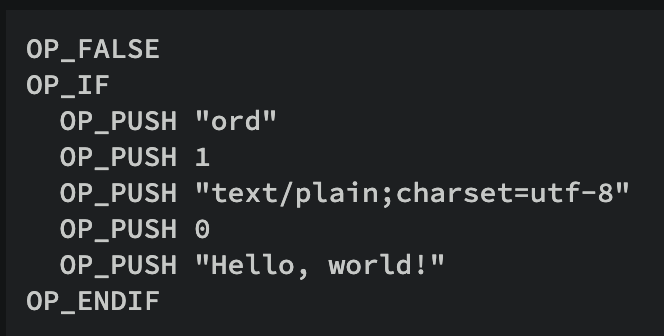
\includegraphics[width=\textwidth]{./assets/ord_enveloppe.png}
  \end{minipage}
  \hfill
  \begin{minipage}[b]{0.51\textwidth}
    \centering
    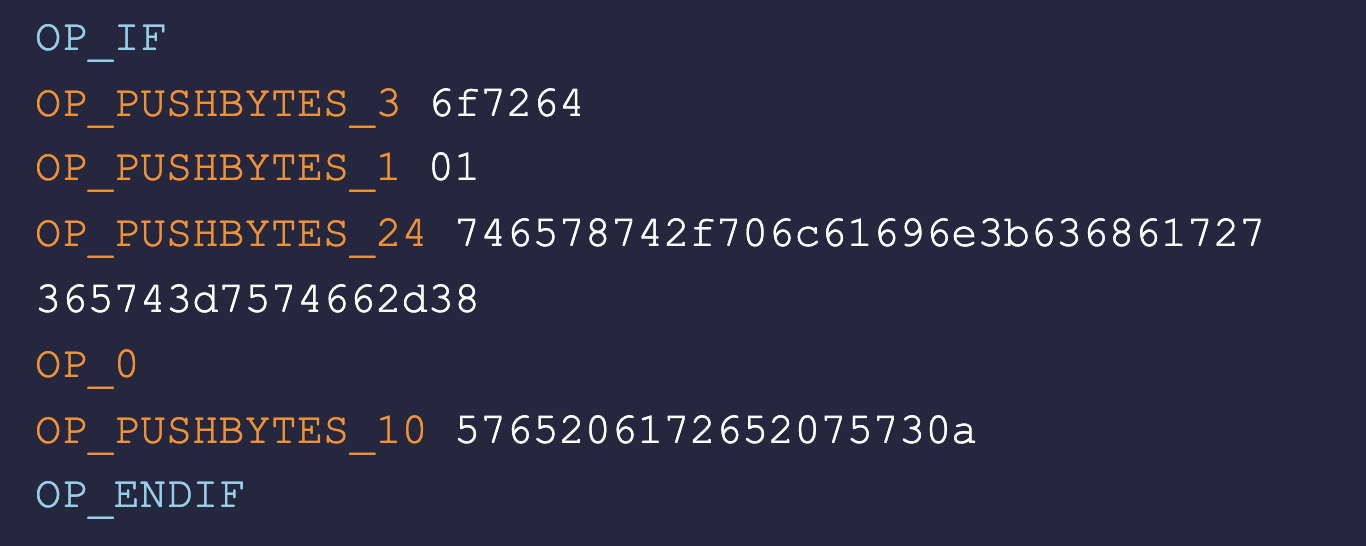
\includegraphics[width=\textwidth]{./assets/ord_tx.png}
  \end{minipage}
  \caption{Ordinals Enveloppe (left) Example of \href{https://mempool.space/tx/58a9c5a603b9dcf4a94ab925764783a0d21f3cf7ee86c02bddfd8b41e0b3da72}{text file inscription} (right)}

\end{figure}

\end{center}
\end{frame}

\begin{frame}
\frametitle{Atomicals Core components}

\begin{center}
{\Large The \href{https://atomicals-community.github.io/atomicals-guide/}{Atomicals protocol} contains three core components}:\\
\vspace{0.3cm}

\begin{itemize}

\item An {\bf ElectrumX implementation}: a fork of ElectrumX named \href{https://github.com/atomicals/atomicals-electrumx}{\texttt{atomicals-electrumx}}. It creates custom electrumx RPC endpoint;\\

\item An {\bf Enveloppe}: built in Bitcoin Script on the same principle of Ordinals~\ref{atom};\\

\item A {\bf Command Line}: built in JavaScript to interact directly with Atomicals protocol. The CLI doesn't manage the indexer.\\

\end{itemize}

\end{center}

\end{frame}

\begin{frame}
\frametitle{Atomicals script enveloppe}

\begin{center}

\begin{figure}
  \label{atom}
  \centering
  \begin{minipage}[b]{0.5\textwidth}
    \centering
    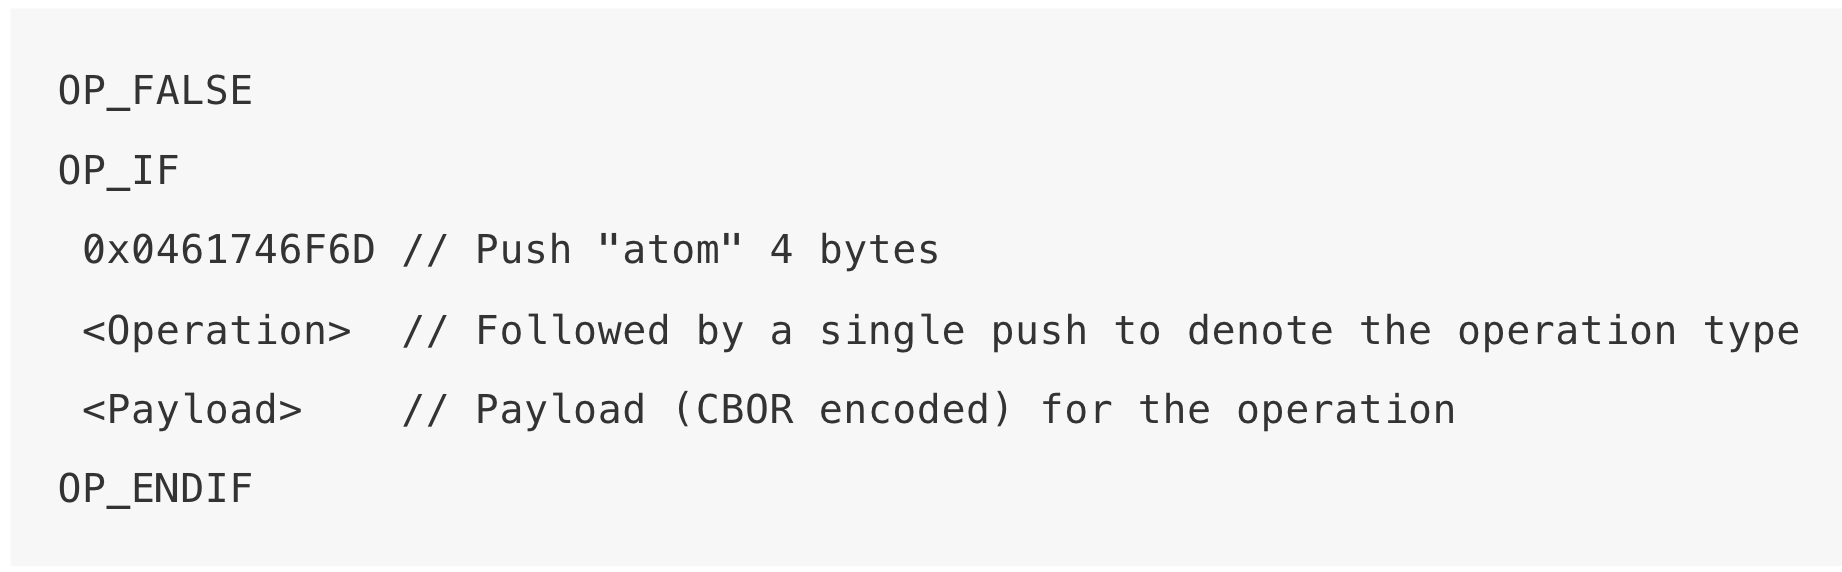
\includegraphics[width=\textwidth]{./assets/atom_enveloppe.png}
  \end{minipage}
  \hfill
  \begin{minipage}[b]{0.45\textwidth}
    \centering
    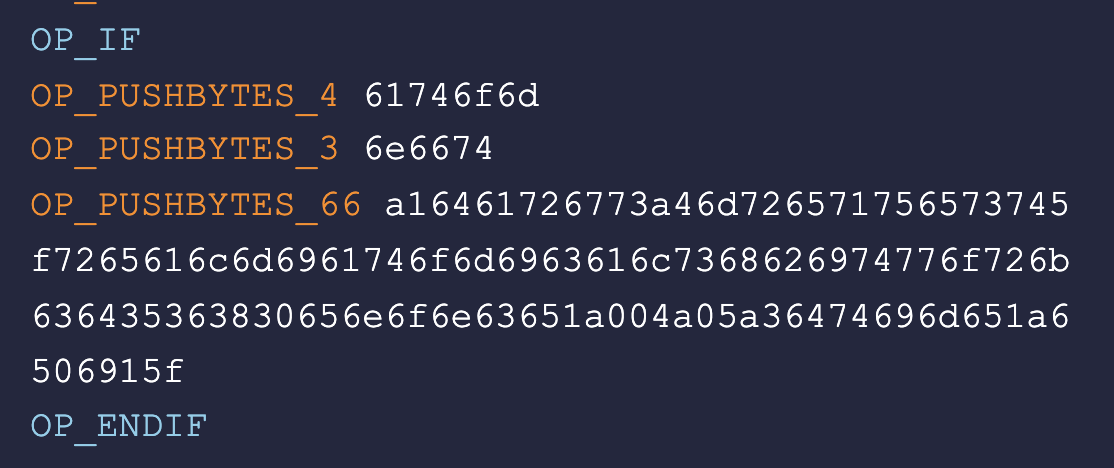
\includegraphics[width=\textwidth]{./assets/atom_tx.png}
  \end{minipage}
  \caption{Atomicals Enveloppe (left) Example of a \href{https://mempool.space/tx/27701d793710cd244a253922e6ef22121d8c78c0a34f2b7b1188cba6f05d4342}{Realm transaction} (right)}

\end{figure}

\end{center}

\end{frame}

%\begin{frame}
%\frametitle{Atomicals Digital Objects}

%\begin{center}
%{\Large The \href{https://atomicals-community.github.io/atomicals-guide/}{Atomicals protocol} contains 3 kind of Digital Objects}:\\
%\vspace{0.3cm}

%\begin{itemize}

%\item {\bf Realms}: an equivalent of Domain Name Service natively built on Bitcoin (as ENS);\\

%\item {\bf NFT} and {\bf containers}: as regular NFT a container is the equivalent of an NFT collection;\\

%\item {\bf Fungible Token}: as ERC-20 standard tokens on Ethereum, they are called ARC-20 tokens.\\

%\end{itemize}

%\end{center}

%\end{frame}




%%%%%%%%%%%%%%%%%%%%%%%%%%%%%%%%%%%%%%%%%%%%%%%%%%%%%%%%%%%%%%%%%%%%%%%%
%%%%%%%%%%%%%%%%%%%%%%%%%%%%%%%%%%%%%%%%%%%%%%%%%%%%%%%%%%%%%%%%%%%%%%%%
% Short title:
\section{3. Mechanisms \& Goals}
%%%%%%%%%%%%%%%%%%%%%%%%%%%%%%%%%%%%%%%%%%%%%%%%%%%%%%%%%%%%%%%%%%%%%%%%
%%%%%%%%%%%%%%%%%%%%%%%%%%%%%%%%%%%%%%%%%%%%%%%%%%%%%%%%%%%%%%%%%%%%%%%%

\begin{frame}
\frametitle{Commit/Reveal}

\begin{center}

Both enveloppe's protocol are using a mechanism of Commit/Reveal transaction. 

\vspace{1cm}

The first commit transaction is made as a \texttt{P2TR} script. The second (reveal) transaction is signing the locking script and adding the enveloppe as shown above.\\

\begin{figure}
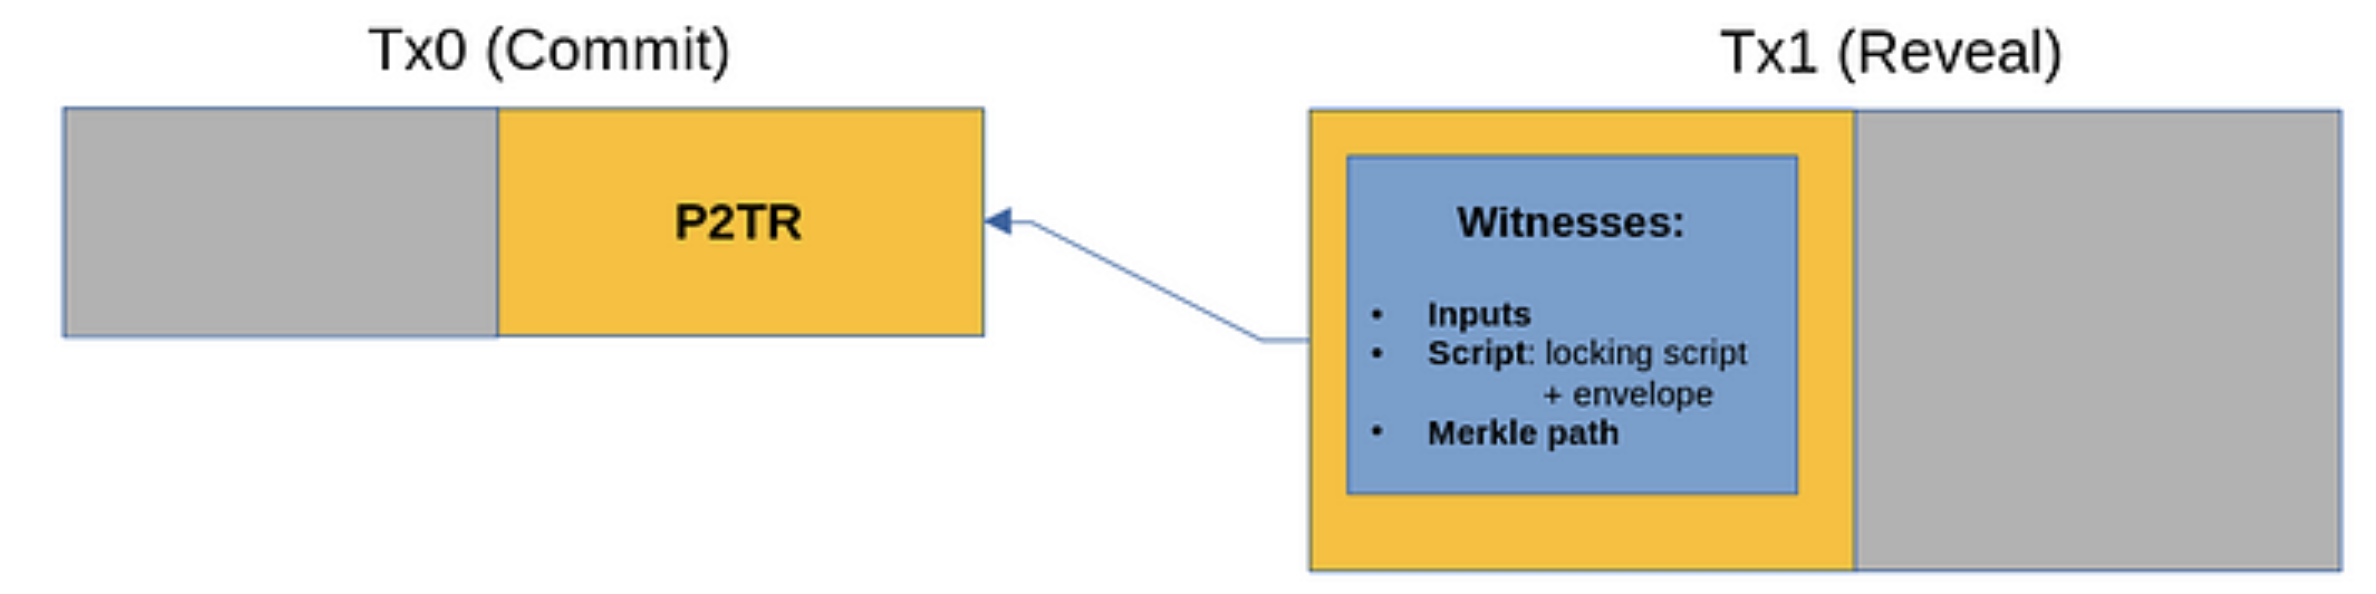
\includegraphics[width=\textwidth]{./assets/commit_reveal.png}
\caption{Commit Reveal Scheme.\\ {\tiny \it source: \href{https://coingeek.com/incorporate-smart-contracts-into-ordinals-on-btc/}{Incorporate smart contracts into Ordinals on BTC - CoinGeek}}}
\end{figure} 

\end{center}

\end{frame}


\begin{frame}
\frametitle{Goals}

\begin{center}

{\Large I purpose a list of current research problems about these protocols}: \\
\vspace{0.3cm}

\begin{itemize}

\item {\bf How can we deploy BLOBs and make calls of them through Enveloppe's protocol?} A first way to achieve it could be to create specific indexer which can integrate specific Virtual Machines for BLOB management as \href{https://www.rgbfaq.com/rgb-paradigms}{RGB};\\

\item {\bf Is it possible to build native bridges between UTXO-based blockchains?} With ordinals protocol on Litecoin and on Dogecoin we can wonder if native bridges are possible in better way than nowadays bridges;\\

\end{itemize}

\end{center}

\end{frame}

\begin{frame}
\frametitle{Goals}

\begin{center}

\begin{itemize}

\item {\bf Create a classification and academic studies of Enveloppes based Protocols.} This will be the first academic work about this kind of Protocols based on Bitcoin. We can easily extend those research to every UTXO-based blockchains. An extension of such classification could be done for Extended-UTXO model used by Cardano.\\

\item {\bf Show optimality of such protocols regarding last \href{https://github.com/bitcoin/bips/blob/master/bip-0341.mediawiki}{Schnorr-Taproot update} (BIP 341).} Some actual considerations tend to show that these protocols aren't optimal. The Taproot upgrade is implementing MAST (Merkelized Alternative Script Trees). Are we able to use MAST to implement and optimise Enveloppe's protocol?  

\end{itemize}

\end{center}

\end{frame}

\begin{frame}

\begin{center}

\begin{figure}

\includegraphics[width=\textwidth]{./assets/blockchain_revolution_technologie_cryptographie_280230556_Drupal.jpg}
\end{figure} 

\end{center}

\end{frame}





\end{document}